% VLDB template version of 2020-08-03 enhances the ACM template, version 1.7.0:
% https://www.acm.org/publications/proceedings-template
% The ACM Latex guide provides further information about the ACM template

\documentclass[sigconf, nonacm]{acmart}
\usepackage[english]{babel}
\usepackage{tikz}
\usepackage{amsmath}
\usepackage{xspace}
\usepackage{makecell}
\usepackage{pifont}
\usepackage{amsfonts}
\usepackage{makecell}
\usepackage[font=small,labelfont=bf]{caption}
% inlined bib file
\usepackage{filecontents}
\usepackage{xurl}
\usepackage{listings}
\usepackage{minted}

\newcommand\sysname{\textsf{CacheKV}\xspace}
\newcommand\redbf{\bf\color{red}}
\renewcommand{\paragraph}[1]{\smallskip\noindent {\bf #1}}
\newcommand\blfootnote[1]{%
  \begingroup
  \renewcommand\thefootnote{}\footnote{#1}%
  \addtocounter{footnote}{-1}%
  \endgroup
}

%% The following content must be adapted for the final version
% paper-specific
\newcommand\vldbdoi{XX.XX/XXX.XX}
\newcommand\vldbpages{XXX-XXX}
% issue-specific
\newcommand\vldbvolume{14}
\newcommand\vldbissue{1}
\newcommand\vldbyear{2020}
% should be fine as it is
\newcommand\vldbauthors{\authors}
\newcommand\vldbtitle{\shorttitle}
% leave empty if no availability url should be set
\newcommand\vldbavailabilityurl{URL_TO_YOUR_ARTIFACTS}
% whether page numbers should be shown or not, use 'plain' for review versions, 'empty' for camera ready
\newcommand\vldbpagestyle{plain}

%-------------------------------------------------------------------------------
\begin{document}
%-------------------------------------------------------------------------------

%don't want date printed
\date{}

% make title bold and 14 pt font (Latex default is non-bold, 16 pt)
\title{CacheKV: Redesigning High-Performance Key-Value Stores with Persistent CPU Caches (Supplemental Material)}
\author{Yijie Zhong}
\affiliation{%
  \institution{Xiamen University}
}
\email{yijiezhong12@gmail.com}

\author{Zhirong Shen}
\affiliation{%
  \institution{Xiamen University}
}
\email{shenzr@xmu.edu.cn}

\author{Zixiang Yu}
\affiliation{%
  \institution{Xiamen University}
}
\email{yuzixiang23@foxmail.com}

\author{Jiwu Shu}
\affiliation{%
  \institution{Tsinghua University, Xiamen University}
}
\email{shujw@tsinghua.edu.cn}
\maketitle



%-------------------------------------------------------------------------------
\section{Summary of Implementations}
%-------------------------------------------------------------------------------

We implement our proposed \sysname atop LevelDB \cite{leveldb} with C++.
We make use of Intel CAT \cite{cat} to allocate space in
the persistent CPU caches. We elaborate on the dependent softwares,
representative KV stores, and testing tool as follows.

\paragraph{Dependent softwares:} the implementation of
\sysname relies on a suit of softwares, including 
{\tt ndctl}, {\tt ipmctl}, {\tt Intel PMWatch}, and {\tt PMDK},
which can be reached via the following URLs.

\begin{minted}{bash}
  $ wget https://github.com/pmem/ndctl
  $ wget https://github.com/intel/ipmctl
  $ wget https://github.com/intel/intel-pmwatch
  $ wget https://github.com/pmem/pmdk
\end{minted}

\paragraph{Representative KV stores:}
we use two representative KV stores for comparison, namely
NoveLSM \cite{kannan18} and SLM-DB \cite{kaiyrakhmet19},
which can be downloaded via the following URLs.

\begin{minted}{bash}
  $ wget https://github.com/sudarsunkannan/lsm_nvm
  $ wget https://github.com/WangEP/SLM-DB
\end{minted}

\paragraph{Testing tools:} we employ {\tt db\_bench} and {\tt YCSB-C}
in our evaluation, where {\tt db\_bench} is released with LevelDB \cite{leveldb}
and YCSB-C \cite{cooper10} is a C++ version of YCSB. They can be
reached via the following URLs.

\begin{minted}{bash}
  $ wget https://github.com/google/leveldb
  $ wget https://github.com/basicthinker/YCSB-C
\end{minted}

%-------------------------------------------------------------------------------
\section{Evaluation Details}
%-------------------------------------------------------------------------------

\paragraph{Hardware configurations:}
We conduct extensive experiments on a single machine
equipped with two 2.10 GHz Intel Golden 5318Y CPUs
(with 24 cores in total), 128 GB of DRAM memory and four
Optane PMem DIMMs of 200 series (128 GB per DIMM and
512 GB in total). The Optane PMem DIMMs are configured
in interleaved {\tt App Direct Mode}, which are connected to one
processor. Figure~\ref{fig:processor} shows the major
hardware configurations of our testbed and
Figure~\ref{fig:pmem} shows detailed information
about the Optane PMem used in our evaluation.

\begin{figure}[t]
\centering
\hspace{-0.1in}
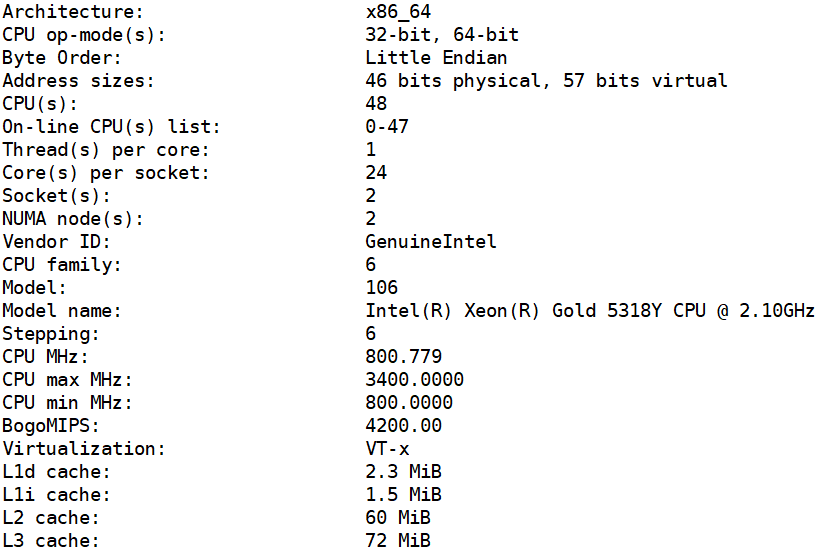
\includegraphics[width=8.5cm]{figures/hardware.png}
\caption{Configurations of our testbed.}
\label{fig:processor}
\end{figure}

\begin{figure}[t]
\centering
\hspace{-0.1in}
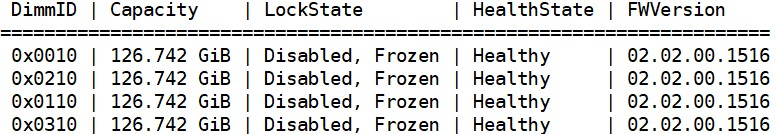
\includegraphics[width=8.5cm]{figures/PMem.jpg}
\caption{The configurations of the Intel Optane PMem DIMMs of 200 series used in
the evaluation.}
\label{fig:pmem}
\end{figure}

We perform extensive testbed experiments, including (i) experiments to understand
the properties of \sysname; and (ii) experiments to understand the sensitivity of \sysname.

\paragraph{Experiments with db\_bench:} 
We measure the access performance of \sysname, NoveLSM, and SLM-DB using {\tt db\_bench}.
The following script runs {\tt db\_bench} to evaluate NoveLSM:
\begin{minted}{bash}
#!/bin/bash
$./db_bench --benchmarks=fillrandom,readrandom
--threads=1 --num=1000000 --value_size=64
--num_levels=2 --nvm_buffer_size=16
\end{minted}

As SLM-DB has realized a {\tt db\_bench} tool for
evaluation, we run the following script to evaluate
SLM-DB with {\tt db\_bench}:
\begin{minted}{bash}
#!/bin/bash
$ ./db_bench --benchmarks=fillrandom,readrandom
--threads=1 --num=1000000 --value_size=64
--nvm_dir=/mnt/pmem0dir-node0/dbbench
\end{minted} 

We amend {\tt db\_bench} to add the configurations required 
in \sysname. The following script is used to evaluate \sysname. 
\begin{minted}{bash}
#!/bin/bash
$./db_bench --threads=1 --num=1000000 
--benchmarks=fillrandom  --value_size=64 
--num_read_threads=1 --dlock_way=4 --dlock_size=12582912 
--subImm_thread=1 --skiplistSync_threshold=65536 
--compactImm_threshold=10 --subImm_partition=0
\end{minted} 

\paragraph{Experiments with YCSB:} 
We also employ YCSB-C as an example to clarify how we assess
the performance of NoveLSM and \sysname. The experiments with
other YCSB workloads are similar.
As SLM-DB is tested by its own {\tt db\_bench} tool that provides an API for YCSB
test, the workload file of SLM-DB can be generated by using the following script:
\begin{minted}{bash}
#!/bin/bash
$./ycsb run basic -P workloada > trace_a.csv
$./db_bench --csv=1 --trace_dir=../trace
--benchmarks=workloada --value_size=64
--nvm_dir=/mnt/pmem0dir-node0/pool
--nvm_size=20480 --threads=1
--db=/mnt/pmem0dir-node0/dbbench
--write_buffer_size=4294967296
\end{minted}


For NoveLSM and \sysname, we can generate the workload file. 
The following script evaluates NoveLSM using the workload 
{\tt YCSB-A}. The scripts to evaluate \sysname with other 
YCSB workloads are similar by modifying the following script. 
\begin{minted}{bash}
#!/bin/bash
$ ./ycsbc -db novelsm -path /mnt/pmem0dir-node0/
-threads 1 -P workloads/workloada.spec
\end{minted}



%The output is in figure \ref{fig:slmdbycsb}.



\bibliographystyle{plain}
\bibliography{paper}
%%%%%%%%%%%%%%%%%%%%%%%%%%%%%%%%%%%%%%%%%%%%%%%%%%%%%%%%%%%%%%%%%%%%%%%%%%%%%%%%
\end{document}
%%%%%%%%%%%%%%%%%%%%%%%%%%%%%%%%%%%%%%%%%%%%%%%%%%%%%%%%%%%%%%%%%%%%%%%%%%%%%%%%

